\chapter{Union-find problém}\label{chap:uf}

V niektorých aplikáciach potrebujeme udržiavať prvky rozdelené do skupín
(disjunktných množín), pričom skupiny sa môžu zlučovať a my potrebujeme
pre daný prvok efektívne zistiť, do ktorej skupiny patrí. Predpokladáme,
že každá množina $S$ je jednoznačne určená jedným svojim zástupcom $x\in S$
a potrebujeme implementovať nasledovné tri operácie:

\begin{itemize}
\item $\makeset(x)$ -- vytvorí novú množinu $S=\{x\}$ s jedným prvkom; %,
                   %ktorý nepatrí do žiadnej inej množiny;
\item $\union(x, y)$ -- ak $x, y$ sú zástupcovia množín $S$ a $T$,
                 $\union$ vytvorí novú množinu $S\cup T$,
                 pričom $S$ aj $T$ zmaže. Zástupcom novej množiny $S\cup T$
                 je $x$ alebo $y$.
\item $\find(x)$ -- nájde zástupcu množiny, v ktorej sa 
                prvok $x$ nachádza.
\end{itemize}
 
\section{Použitie}\label{sec:uf-pouzitie}

Union-find sa dá použiť na reprezentáciu neorientovaného grafu,
do ktorého pridávame hrany a odpovedáme na otázku: "Sú dané dva
vrcholy spojené nejakou cestou?" (t.~j.\ sú v rovnakom komponente súvislosti?)
Medzi najznámejšie aplikácie patria Kruskalov algoritmus na nájdenie najlacnejšej
kostry \citep{kruskal} a unifikácia \citep{unif}.

\citet{cholesky} ukázali, ako sa dá union-find použiť pri Choleského dekompozícií
riedkych matíc. Autori navrhli efektívny algoritmus, ktorý zistí počet nenulových
prvkov v každom riadku a stĺpci výslednej matice, čo slúži na efektívnu alokáciu
pamäte.

Pre offline verziu úlohy, kde sú všetky operácie dopredu známe, \citet{offline-uf}
navrhli lineárny algoritmus. Článok obsahuje tiež viacero aplikácií v teoretickej
informatike.

\section{Popis}
Dátová štruktúra \emph{union-find} sa reprezentuje ako les, kde každý strom zodpovedá
jednej množine a korene stromov sú zástupcovia množín. Pri implementácií si
stačí pre každý prvok $x$ udržiavať smerník $p(x)$ na jeho otca
(pre koreň je $p(x)=\nul$).

Operácia $\makeset(x)$ teda vytvorí nový prvok $x$ a nastaví $p(x) = \nul$. 

Operáciu $\find(x)$ vykonáme tak, že budeme sledovať cestu po smerníkoch, až 
kým nenájdeme zástupcu. 

Operáciu $\union(x, y)$ ide najjednoduchšie vykonať tak, že presmerujeme smerník 
$p(y)$ na prvok $x$, teda $p(y) \gets x$. 
Môžeme ľahko pozorovať, že takýto \emph{naivný} spôsob je neefektívny, 
lebo nám operácia $\find(x)$ v najhoršom prípade, na $n$ prvkoch, trvá $\Omega(n)$ 
krokov. 

\smallskip
Existujú dva prístupy ako zlepšiť operácie a tým aj zrýchliť ich vykonanie. 
Sú to: heuristika \emph{spájanie podľa ranku} a rôzne heuristiky na 
\emph{kompresiu cesty}. 

\section{Heuristika na spájanie}\label{sec:komp-union}

Prvá heuristika pre každý vrchol $x$ udržuje hodnotu $\rank(x)$,
ktorá určuje najväčšiu možnú hĺbku podstromu s koreňom $x$.
Pri o\-pe\-rá\-cií $\makeset(x)$ zadefinujeme $\rank(x) = 1$. 
Pri o\-pe\-rá\-cií $\union(x, y)$ porovnáme $\rank(x)$ a $\rank(y)$
a vždy napojíme strom s menším rankom pod strom s väčším rankom.
Ak majú oba stromy rovnaký rank, napojíme povedzme $x$ pod $y$
a $\rank(y)$ zvýšime o 1.
%aby sme zistili, ktorý zástupca predstavuje menší strom. 
% Smerník tohto zástupcu potom napojíme 
% na zástupcu s výšším rankom. Zástupca novej množiny bude ten s vyšším rankom. 
% Ak sú oba ranky rovnaké, vyberieme ľubovoľného zo zástupcov $x$ a $y$, 
% jeho rank zvýšime o jeden a smerník ostatného zástupcu bude ukazovať 
% na tohto zástupcu. %Zástupcom novej množiny bude vybratý zástupca. 

\section{Heuristiky na kompresiu cesty}\label{sec:komp-cesta}
      
\begin{figure}
\centering
\subfloat[Pred vykonaním kompresie.]{
\label{img:komp1}
% ,width=0.4\textwidth
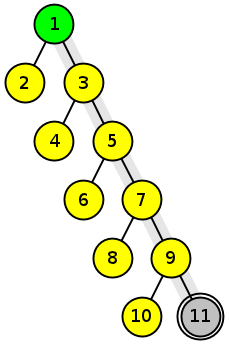
\includegraphics[height=0.24\textheight]{obrazky/komp1.png}
}
\qquad
\subfloat[Úplná kompresia.]{
\label{img:komp2}
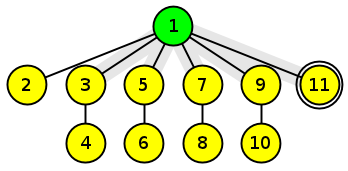
\includegraphics[height=0.12\textheight]{obrazky/komp2.png}
}

\subfloat[Delenie cesty.]{
\label{img:komp3}
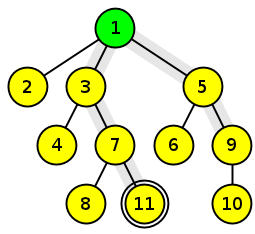
\includegraphics[height=0.16\textheight]{obrazky/komp3.png}
}
\qquad
\subfloat[Pólenie cesty.]{
\label{img:komp4}
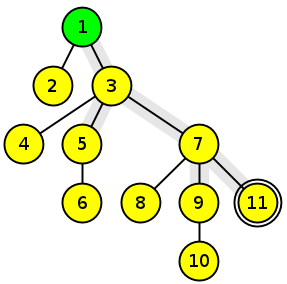
\includegraphics[height=0.20\textheight]{obrazky/komp4.png}
}
 
\label{img:kompresia}
\caption{\emph{Kompresia cesty z vrcholu 11 do koreňa.} 
Cesta je vyznačená šedou. 
Pri úplnej kompresii~\subref{img:komp2} sa všetky vrcholy 
napoja na zástupcu. Pri delení cesty~\subref{img:komp3} a pólení 
cesty~\subref{img:komp4} sa cesta skráti približne na polovicu.}
\end{figure}
 
Druhou heuristikou je kompresia cesty. Algoritmov na efektívnu kompresiu 
cesty je veľa \citep{paths2}, tu popíšeme tie najefektívnejšie. Prvou z nich 
je \emph{úplná kompresia} \citep{comp1}. Pri vykonávaní operácie $\find(x)$, po 
tom, ako nájdeme zástupcu, napojíme všetky vrcholy po ceste priamo pod koreň 
(obr.~\ref{img:komp2}). Toto síce trochu spomalí prvé hľadanie, ale výrazne 
zrýchli ďalšie hľadania pre všetky prvky na ceste ku koreňu. Druhou 
heuristikou je \emph{delenie cesty} \citep{comp2}. Pri vykonávaní operácie 
$\find(x)$ pripojíme každý vrchol v ceste od vrcholu $x$ po koreň stromu na otca 
jeho otca (obr.~\ref{img:komp3}). Treťou heuristikou je \emph{pólenie cesty} 
\citep{comp2}. Pri vykonávaní operácie $\find(x)$  pripojíme každý druhý vrchol 
v ceste od vrcholu $x$ po koreň stromu na otca jeho otca 
(obr.~\ref{img:komp4}).

Časová zložitosť union-findu záleží od toho, koľko prvkov je v množinách a koľko je 
operácií celkovo vykonaných operácií. Všetky uvedené spôsoby ako vykonať 
operáciu $\find(x)$ sa dajú použiť s obomi realizáciami operácie $\union$. 
Počet prvkov označme $n$ a počet operácií $m$. V praxi je zvyčajne počet 
operácií oveľa väčší ako počet prvkov. Pri tomto predpoklade ($m\geq n$) je 
pri použití spájania podľa ranku časová zložitosť pre algoritmus bez kompresie 
$\Theta(m\log n)$ a pre všetky tri uvedené typy kompresií 
$\Theta(m\mathop{\alpha}(m,n))$. 
V tabuľke~\ref{fig:uf:comp} je porovnanie časových zložitostí \citep{paths2}.

\begin{table}
\centering
\small
%\footnotesize %toto tu mám nechať?
\subfloat[Časová zložitosť pre union-find, keď $m \geq n$.][Prehľad časových zložitostí, ak $m \geq n$.]{
\begin{tabular}{m{5cm}m{4cm}m{4cm}}
& Naivné spájanie & Spájanie podľa ranku \tabularnewline
\hline
Naivné hľadanie & $\Theta\left( mn\right)$ & $\Theta\left( m\log n\right)$ \tabularnewline
Úplná kompresia, delenie cesty, pólenie cesty & $\Theta\left(m\log _{1+m/n} n \right)$ & $\Theta\left( m\alpha\left( m, n\right) \right)$ \tabularnewline
\label{fig:uf:comp1}
\end{tabular}
}
\qquad
\subfloat[Časová zložitosť pre union-find, keď $m < n$.][Prehľad časových zložitostí, ak $m < n$.]{
\begin{tabular}{m{5cm}m{4cm}m{4cm}}
& Naivné spájanie & Spájanie podľa ranku \tabularnewline
\hline
Naivné hľadanie & $\Theta\left( mn\right)$ & $\Theta\left(n + m\log n\right)$ \tabularnewline
Úplná kompresia& $\Theta\left(n + m\log  n \right)$ & $\Theta\left(n + m\alpha\left( n, n\right) \right)$ \tabularnewline
Delenie cesty & $\Theta\left(n \log m \right)$ & $\Theta\left(n + m\alpha\left( n, n\right) \right)$ \tabularnewline
Pólenie cesty & $\Omega\left(n + m\log n \right)$, $O\left(n\log m\right)$ & $\Theta\left(n + m\alpha\left( n, n\right) \right)$ \tabularnewline
\label{fig:uf:comp2}
\end{tabular}}
\caption{\normalsize Porovnanie časových zložitostí pre rôzne kombinácie hľadaní prvkov a 
spájaní množín pre union-find. Počet prvkov je $n$ a počet operácií je $m$. 
Ackermannova inverzná funkcia je označená ako $\alpha$. V praxi zväčša platí, že $m > n$.}
\label{fig:uf:comp}
\end{table}

% \section{Vizualizácia}
% Dátovú štruktúru union-find sme vizualizovali ako les. Pre názorné 
% oddelenie množín sme si zvolili pravidlo, ktoré zakazovalo vykresliť vrchol 
% z iného stromu (prvok inej množiny) 
% napravo od najľavejšieho vrcholu a naľavo od napravejšieho vrcholu inej 
% množiny. Jednotlivé množiny sme už vykreslovali tesným Walkerovým algoritmom 
% \citep{walker}. Vizualizácia poskytuje všetky vyššie spomínané heuristiky a 
% aj tlačidlo na vykonanie viacerých náhodných spojení naraz. Toto je užitočné, 
% keď chce uživateľ vidieť, ako dátová štruktúra vyzerá, po vykonaní 
% veľa operácií.
% 

